\section{Doxyblocks}\label{sec:doxyblocks}

DoxyBlocks est une extension pour \codeblocks qui intègre doxygen dans l'IDE. Il vous permet de créer de la documentation, insérer des blocs de commentaires et de lancer des documents HTML ou CHM. Il fournit également la configuration de quelques-uns des paramètres les plus communément utilisés at un accès à doxywizard pour obtenir une configuration plus détaillée.

Les paramètres de la barre d'outils de DoxyBlocks ont la signification suivante :

\begin{description}
\item[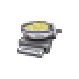
\includegraphics{Doxywizard}] Lancer doxywizard. Ctrl-Alt-D
\item[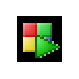
\includegraphics{Extract}] Extraire la documentation du projet courant. Ctrl-Alt-E
\item[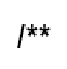
\includegraphics{Comment_block}] Insère un bloc de commentaires sur la ligne courante. De plus, DoxyBlocks essaiera de façon intelligente de lire si une méthode existe dans la ligne où le commentaire est en train d'être ajouté. Ctrl-Alt-B

\begin{lstlisting}
/** \brief
 *
 * \param bar bool
 * \return void
 *
 */    
void MyClass::Foo(bool bar)
{
    fooBar(bar);
}
\end{lstlisting}

\item[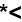
\includegraphics{Comment_line}] Insère une ligne de commentaire à la position actuelle du curseur. Ctrl-Alt-L
\begin{lstlisting}
void MyClass::Foo(bool bar)
{
    fooBar(bar); /**<  */
}
\end{lstlisting}

\item[
\includegraphics{Html}] Affiche la documentation HTML générée. Ctrl-Alt-H
\item[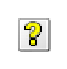
\includegraphics{Chm}] Affiche la documentation CHM (Help) générée. Ctrl-Alt-C
\item[
\includegraphics{Configure}] Ouvre les préférences de DoxyBlocks. Ctrl-Alt-P
\end{description}

Doxyblocks ne peut travailler que si doxygen est installé sur votre système. Vous avez besoin au moins des exécutables de doxygen et de doxywizard (disponibles dans la distribution officielle de doxygen sur \url{http://www.doxygen.nl/}). En option, vous pouvez avoir l'exécutable "dot" du package graphviz (voir \url{https://graphviz.gitlab.io/}. Sous Windows, le compilateur d'aide (hhc) peut également être utilisé les fichiers de type chm.

\genterm{Notes}
\begin{description}
\item Dans les préférences, vous avez une case à cocher qui autorise ou pas DoxyBlocks à \textbf{écraser le fichier doxyfile}. Par défaut, si un doxyfile existe déjà il ne sera pas écrasé pour protéger de divers changements qui auraient pu être faits en dehors de DoxyBlocks. Néanmoins ce comportement empèche aux changements faits par DoxyBlocks lui-même d'être écrits dans le doxyfile existant.
\item Si un champ de texte des "Préférences" est vide, DoxyBlocks assumera que l'exécutable correspondant est disponible quelquepart via votre variable d'environnement path. Vous pouvez utiliser des macros telles que \$(CODEBLOCKS) dans votre path et elles seront automatiquement étendues.
\item [OUTPUT\_DIRECTORY] Utilisé pour spécifier le chemin de base (relatif ou absolu) ou sera enregistrée la documentation générée. Si un chemin relatif est entré, il sera en relatif par rapport à l'emplacement d'où doxygen a été lancé. Si laissé en blanc, c'est le répertoire courant qui sera utilisé. Doxyblocks utilisera le nom de chemin entré ici pour créer un répertoire relatif au \codeline{<rep. projet>}. Ceci vout permet de créer des répertoire doxygen différents pour des projets inclus dans un même répertoire, ou simplement utiliser un nom de répertoire différent. Si le champ est laissé en blanc, les documents seront créés dans "\codeline{<rep. projet>/doxygen}". Entrer les noms de répertoires sans points, ni séparateurs de tête, ni nom de volume, etc. DoxyBlocks effectue la validation sur le nom de chemin et supprime les caractères en trop.
\begin{code}
Exemples:
[blanc]           -> <répertoire projet>/doxygen.
"docs"            -> <répertoire projet>/docs.
"docs/sub1/sub2"  -> <répertoire projet>/docs/sub1/sub2.
"doxygen/docs"    -> <répertoire projet>/doxygen/docs.
\end{code}
\item [OUTPUT\_LANGUAGE]  Utilisé pour spécifier dans quelle langue sera générée la documentation par doxygen. Doxygen utilisera cette information pour générer toutes les sorties constantes dans la langue adéquate. La langue par défaut est l'anglais. D'autres langues sont supportées. 
\item D'autres informations dans les fichiers d'aide de doxygen
\end{description}